\documentclass[12pt,a4paper]{article}

%=========
% PACKAGES
%=========

\usepackage{graphicx}
\usepackage[section]{placeins}
\usepackage{float}
\usepackage{amsmath}
\usepackage{listings}
\usepackage{xcolor}
\usepackage{extarrows}
\usepackage{verbatim}
\usepackage{enumerate}
\usepackage{enumitem}
\usepackage{eurosym}
\usepackage{svg}
\usepackage{varwidth}
\usepackage{moreverb}
\usepackage{relsize}
\usepackage{tabto}
\usepackage[margin=1in]{geometry}
\usepackage[normalem]{ulem}
\usepackage{units}
\usepackage{fancyvrb}
\usepackage{fontspec}
\usepackage{extarrows}
\usepackage{amsfonts}
\usepackage{amssymb}
\usepackage{hyperref}
%\usepackage{unicode-math}


%=====================
% SETTINGS/DEFINITIONS
%=====================

% Don't break words with hyphens. Instead, wrap word to next line.
\tolerance=1
% \emergencystretch=\maxdimen
\hyphenpenalty=10000
\hbadness=10000

\definecolor{codegreen}{rgb}{0,0.6,0}
\definecolor{codegray}{rgb}{0.5,0.5,0.5}
\definecolor{codepurple}{rgb}{0.58,0,0.82}
\definecolor{backcolour}{rgb}{0.95,0.95,0.92}

\def\verbatimtabsize{4}

\lstdefinestyle{mystyle}{
	backgroundcolor=\color{backcolour},
	commentstyle=\color{codegreen},
	keywordstyle=\color{magenta},
	numberstyle=\tiny\color{codegray},
	stringstyle=\color{codepurple},
	basicstyle=\ttfamily\footnotesize,
	breakatwhitespace=false,
	breaklines=true,
	captionpos=b,
	keepspaces=true,
	numbers=left,
	numbersep=5pt,
	showspaces=false,
	showstringspaces=false,
	showtabs=false,
	tabsize=2
}

\lstset{style=mystyle}

\setlength{\parindent}{0pt}
\setlength{\parskip}{0em}
\setlength{\jot}{4mm}

\pagenumbering{gobble}

\hypersetup{
    colorlinks=true,
    linkcolor=blue,
    filecolor=blue,      
    urlcolor=blue,
}

\setmainfont{Minion Pro}

\newcommand{\imagesPath}{/home/nick/shmmy/8th/slp/slp-ntua/set1}

\title{Επεξεργασία Φωνής και Φυσικής Γλώσσας \\ 1η σειρά αναλυτικών ασκήσεων}
\author{Νικόλαος Παγώνας, el18175}
\date{}

\begin{document}
	\maketitle	
	
	\subsection*{Άσκηση 1}
		
		\subsubsection*{1.} 
			Έχουμε: 
			
			\begin{align*}
				y(n) &= \sum_{k=-\infty}^{\infty}v(k) \cdot h_2(n-k) \\
				&= \sum_{k=-\infty}^{\infty}\left[\left(\sum_{\ell=-\infty}^{\infty}x(\ell) \cdot h_1(k-\ell)\right) \cdot h_2(n-k)\right] \\
			\end{align*}
		
			Κάνουμε αλλαγή μεταβλητής $m = k - \ell$ για να αντικαταστήσουμε το $k$:
			
			\begin{align*}
				y(n) &= \sum_{m=-\infty}^{\infty}\left[\left(\sum_{\ell=-\infty}^{\infty}x(\ell) \cdot h_1(m)\right) \cdot h_2(n-\ell-m)\right] \\
				&= \sum_{\ell=-\infty}^{\infty}\left[x(\ell) \cdot \left(\sum_{m=-\infty}^{\infty}h_1(m) \cdot h_2(n-\ell-m)\right)\right] \\
				&= \sum_{\ell=-\infty}^{\infty}x(\ell) \cdot \left(h_1 \ast h_2\right)(n-\ell) \\
				&= x(n) \ast (h_1 \ast h_2)(n) \\
				&= x(n) \ast h(n),
			\end{align*}
		
		όπου $h(n) = h_1(n) \ast h_2(n)$.

		\subsubsection*{2.} 
		
			Έχουμε:
			
			\begin{align*}
				h_1(n) \ast h_2(n) &= \sum_{k=-\infty}^{\infty}h_1(k) \cdot h_2(n-k) \\
			\end{align*}
		
			Κάνουμε αλλαγή μεταβλητής $m = n - k$ για να αντικαταστήσουμε το $k$:
			
			\begin{align*}
				h_1(n) \ast h_2(n) &= \sum_{m=-\infty}^{\infty}h_2(m) \cdot h_1(n-m) \\
				&= h_2(n) \ast h_1(n).
			\end{align*}
		
		\subsubsection*{3.}
			\begin{align*}
				H(z) = H_1(z) \cdot H_2(z) &= \dfrac{Y(z)}{X(z)} \implies \\
				\dfrac{Y(z)}{H_2(z)} &= H_1(z) \cdot X(z) \implies \\
				\left(1-\sum_{k=1}^{N}a_k \cdot z^{-k}\right) \cdot Y(z) &= \left(\sum_{r=0}^{M}b_r \cdot z^{-r}\right) \cdot X(z) 
			\end{align*}
		
			και επειδή: 
			
			\[
				\mathcal{Z}\left[x(n-n_0)\right]=z^{-n_0} \cdot X(z)
			\]
			
			η εξίσωση (μετά από εφαρμογή αντίστροφου Z μετασχηματισμού) γίνεται:
			
			\[
				y(n) - \sum_{k=1}^{N} a_k \cdot y(n-k) = \sum_{r=0}^{M} b_r \cdot x(n-r)
			\]
			
		\subsubsection*{4.}
			Αντίστοιχα:
			
			\begin{align*}
				H(z) = H_2(z) \cdot H_1(z) &= \dfrac{Y(z)}{X(z)} \implies \\ 
				\dfrac{Y(z)}{H_2(z)} &= H_1(z) \cdot X(z)
			\end{align*}
		
			η συνέχεια είναι πανομοιότυπη με το ερώτημα 3.
			
	\subsection*{Άσκηση 2}
		
		\subsubsection*{1.}
			Έχουμε:
			
			\begin{align*}
				R_n(-k) = \sum_{m=-\infty}^{\infty}x(m) \cdot w(n-m) \cdot x(m-k) \cdot w(n+k-m)
			\end{align*}
		
			Κάνουμε την αλλαγή μεταβλητής $\ell=m-k$ για να αντικαταστήσουμε το $m$:
			
			\begin{align*}
				R_n(-k) &= \sum_{\ell=-\infty}^{\infty}x(\ell+k) \cdot w(n-k-\ell) \cdot x(\ell) \cdot w(n-\ell) \\
				&= \sum_{\ell=-\infty}^{\infty}x(\ell) \cdot w(n-\ell) \cdot x(\ell+k) \cdot w(n-k-\ell) \~\~\ \text{   (αναδιάταξη όρων)} \\
				&= R_n(k). 
			\end{align*}
			
		\subsubsection*{2.}
			Έχουμε:
			
			\begin{align*}
				R_n(k) &\overset{1.}{=} R_n(-k) \\
				&\overset{\text{def}}{=} \sum_{m=-\infty}^{\infty} x(m) \cdot w(n-m) \cdot x(m-k) \cdot w(n+k-m) \\
				&= \sum_{m=-\infty}^{\infty} x(m) \cdot x(m-k) \cdot w(n-m) \cdot w(n-m+k) \\
				&= \sum_{m=-\infty}^{\infty} x(m) \cdot x(m-k) \cdot h_k(n-m)
			\end{align*}
					
		\subsubsection*{3.} 
			Είναι:
			
			\begin{align*}
				w(n) = a^n \cdot u(n),				
			\end{align*}
			
			
			όπου $u(n)$ η μοναδιαία βηματική συνάρτηση. Έτσι:
			
			\begin{align*}
				h_k(n) &= w(n) \cdot w(n+k) = a^{2n+k} \cdot u(n) \cdot u(n+k) \\
				h_k(n) &= 
					\begin{cases}
						a^{2n+k} \cdot u(n),~~~~~~~~~~~ k \geq 0 \\
						a^{2n+k} \cdot u(n+k), ~~~ k < 0
					\end{cases}
			\end{align*}
		
		\subsubsection*{4.} 
			Για $k \geq 0$:
			
			\begin{align*}
				h_k(n) = a^{2n+k} \cdot u(n) = a^k \left(a^2\right)^n \cdot u(n) \xrightarrow{\mathcal{Z}} a^k \dfrac{z}{z-a^2}, \ |z| > |a^2| 
			\end{align*}
			
			Για $k < 0$:
			
			\begin{align*}
				h_k(n) = a^{2n+k} \cdot u(n+k) = a^n \cdot \{a^{n+k} \cdot u(n+k)\}
			\end{align*}
			
			Θέτουμε $x(n) = a^n \cdot u(n)$ και εφαρμόζουμε τις δύο ιδιότητες:
			
			\begin{itemize}
				\item $x(n+k) \xrightarrow{\mathcal{Z}} z^k \cdot X(z)$
				\item $a^n \cdot x(n) \xrightarrow{\mathcal{Z}} X\left(\dfrac{z}{a}\right)$
			\end{itemize}

			οπότε προκύπτει 
			
			\begin{align*}
				\mathcal{Z}\left\{h_k(n)\right\} &= \left(\dfrac{z}{a}\right)^k \dfrac{z/a}{z/a-a} \implies \\
				\mathcal{Z}\left\{h_k(n)\right\} &= a^{-k}\dfrac{z^{k+1}}{z-a^2}, \ |z| > |a^2|
			\end{align*}

		Τώρα θα εκφράσουμε το $R_n(k)$ με αναδρομική σχέση βάσει του $h_k(n)$. Έχουμε: \\
		
		Για $k \geq 0$:
		
		\begin{align*}
			h_k(n+1) - a^2 \cdot h_k(n) &= a^{2n+2+k} \cdot u(n+1) - a^{2n+2+k} \cdot u(n) \\
			&= a^{2n+2+k} \cdot (u(n+1) - u(n)) \\ 
			&= a^{2n+2+k} \cdot \delta(n+1), \text{~~~~~~~~~~~~~~~~~~αφού } u(n+1) - u(n) = \delta(n)\\
			&= a^k \cdot \delta(n+1), \text{~~~~~~~~~~~~~~~~~~~~~~~~~~~~αφού } x(n) \cdot \delta(n-n_0) = x(n_0) \cdot \delta(n-n_0)
		\end{align*}
		
		Επομένως:
		
		\[
			h_k(n+1) = a^k \cdot \delta(n+1) + a^2 \cdot h_k(n)
		\]
		
		Για $k < 0$:
		
		\begin{align*}
			h_k(n+1) - a^2 \cdot h_k(n) &= a^{2n+2+k} \cdot u(n+k+1) - a^{2n+2+k} \cdot u(n+k) \\
			&= a^{2n+2+k} \cdot (u(n+k+1) - u(n+k)) \\ 
			&= a^{2n+2+k} \cdot \delta(n+k+1)\\
			&= a^{-k} \cdot \delta(n+k+1)
		\end{align*}
		
		Επομένως:
		
		\[
			h_k(n+1) = a^{-k} \cdot \delta(n+k+1) + a^2 \cdot h_k(n)
		\]

		Για την $R_n(k)$ έχουμε:
		
		\begin{align*}
			R_{n+1}(k) &= \sum_{m=-\infty}^{\infty} x(m) \cdot x(m-k) \cdot h_k(n-m+1) \\
		\end{align*}

		Για $k \geq 0$:
		
		\begin{align*}
			R_{n+1}(k) &= \sum_{m=-\infty}^{\infty} x(m) \cdot x(m-k) \cdot \left[a^k \cdot \delta(n-m+1) + a^2 \cdot h_k(n-m)\right] \\
			&= \sum_{m=-\infty}^{\infty} \left[x(m) \cdot x(m-k) \cdot a^k \cdot \delta(n-m+1)\right] + a^2 \cdot R_n(k) \\
			&= x(n+1) \cdot x(n+1-k) \cdot a^k + a^2 \cdot R_n(k)
		\end{align*}
		
		Για $k < 0$:
		
		\begin{align*}
			R_{n+1}(k) &= \sum_{m=-\infty}^{\infty} x(m) \cdot x(m-k) \cdot \left[a^{-k} \cdot \delta(n-m+k+1) + a^2 \cdot h_k(n-m)\right] \\ 
			&= \sum_{m=-\infty}^{\infty} \left[x(m) \cdot x(m-k) \cdot a^{-k} \cdot \delta(n-m+k+1)\right] + a^2 \cdot R_n(k) \\ 
			&= x(n+k+1) \cdot x(n+1) \cdot a^{-k} + a^2 \cdot R_n(k)
		\end{align*}
		
		Στην πραγματικότητα τα παραπάνω βήματα για $k < 0$ μπορούν να παραλειφθούν, διότι θα μπορούσαμε λόγω της άρτιας συμμετρίας να πούμε ότι:
		
		\[
			R_{n+1}(k) = R_{n+1}(-k) \xlongequal{-k > 0} x(n+1) \cdot x(n+1+k) \cdot a^{-k} + a^2 \cdot R_n(k) 
		\] 
		
		επομένως ο τύπος για $k \geq 0 $ μπορεί να επεκταθεί και για $k < 0$, οπότε ισχύει για $k \in \mathbb{Z}$.
		
		\subsubsection*{5.} 
			Έχουμε:
			
			\begin{align*}
				h_k(n) &= w(n) \cdot w(n+k)  \\
				&= n \cdot a^n \cdot u(n) \cdot (n+k) a^{n+k} \cdot u(n+k) \\
				&= 
					\begin{cases}
						n(n+k) \cdot a^{2n+k} \cdot u(n), ~~~~~~~~~~~ k \geq 0 \\
						n(n+k) \cdot a^{2n+k} \cdot u(n+k), ~~~ k < 0
					\end{cases}
			\end{align*}
			
			Για τον μετασχηματισμό Z έχουμε: \\
			
			Για $k \geq 0$:
			
			\begin{align*}
				h_k(n) &= n(n+k)a^{2n+k} \cdot u(n) \\
				&= n^2a^{2n+k} \cdot u(n) + k \cdot n \cdot a^{2n-k} \cdot u(n) \\
				&= a^k \cdot n \cdot n \cdot \left(a^2\right)^n \cdot u(n) + ka^k \cdot n \cdot \left(a^2\right)^n \cdot u(n) \\
			\end{align*}
			
			Χρησιμοποιώντας τις ιδιότητες:
			
			\begin{itemize}
				\item $ n \cdot x(n) \xrightarrow{\mathcal{Z}} -z\dfrac{dX(z)}{dz}$
				\item $ n \cdot a^n \cdot u(n) \xrightarrow{\mathcal{Z}} \dfrac{az}{(z-a)^2}, ~~~|z| > |a|$
			\end{itemize}
			
			Έχουμε:
			
			\begin{align*}
				\mathcal{Z}\left\{h_k(n)\right\} &= a^k\left\{-z\dfrac{d}{dz}\left[\dfrac{a^2z}{\left(z-a^2\right)^2}\right]+ka^k\dfrac{a^2z}{\left(z-a^2\right)^2}\right\} \\
				&= \dfrac{(1+k) \cdot a^{k+2}z^2+(1-k) \cdot a^{k+4}z}{\left(z-a^2\right)^3}, ~~~~~|z| > |a^2|
			\end{align*}
			
			Για $k < 0$:
			
			\begin{align*}
				h_k(n) &= n \cdot (n+k) \cdot a^{2n+k} \cdot u(n+k) \\
				&= a^k \cdot n \cdot \left(a^2\right)^n \cdot (n+k) \cdot u(n+k)
			\end{align*}
			
			Θέτουμε \begin{align*}
				x_1(n) &= n \cdot u(n) \\
				x_2(n) &= x_1(n+k) \\
				x_3(n) &= \left(a^2\right)^n \cdot x_2(n) 
			\end{align*}
			
			και με βάση τις ιδιότητες:
			
			\begin{itemize}
				\item $x(n+k) \xrightarrow{\mathcal{Z}} z^k \cdot X(z)$
				\item $a^n \cdot x(n) \xrightarrow{\mathcal{Z}} X\left(\dfrac{z}{a}\right)$
				\item $ n \cdot x(n) \xrightarrow{\mathcal{Z}} -z\dfrac{dX(z)}{dz}$
			\end{itemize}
			
			έχουμε:
			
			\begin{align*}
				\mathcal{Z}\left\{h_k(n)\right\} = a^k\left(-z\dfrac{d}{dz}X_3(z)\right) 
			\end{align*}
			
			και επειδή:
			
			\begin{align*}
				X_3(z) &= X_2\left(\dfrac{z}{a^2}\right) \\
				X_2(z) &= z^k \cdot X_1(z) \\
				X_1(z) &= \dfrac{z}{(z-1)^2} \\
			\end{align*}
			
			έχουμε:
			
			\begin{align*}
				X_3(z) = a^{2-2k} \cdot \dfrac{z^{k+1}}{\left(z-a^2\right)^2}
			\end{align*}
			
			και έτσι μετά την εκτέλεση της παραγώγισης προκύπτει:
			
			\begin{align*}
				\mathcal{Z}\left\{h_k(n)\right\} = -a^{2-k} \cdot \dfrac{(k-1)z^{k+2}-a^2(k+1)z^{k+1}}{\left(z-a^2\right)^2}, ~~~~~|z| > |a^2|
			\end{align*}

			Τώρα θα εκφράσουμε το $R_n(k)$ με αναδρομική σχέση βάσει του $h_k(n)$. Έχουμε: \\
			
			Για $k \geq 0$:
			
			\begin{align*}
				h_k(n+1) - \dfrac{(n+1)(n+k+1)}{n(n+k)}a^2 \cdot h_k(n) &= \\  (n+1)(n+k+1) \cdot a^{2n+2+k} \cdot u(n+1)-(n+1)(n+k+1)a^{2n+2+k} \cdot u(n) &= \\
				(n+1)(n+k+1) \cdot a^{2n+2+k} \cdot \left[u(n+1)-u(n)\right] &= \\
				(n+1)(n+k+1) \cdot a^{2n+2+k}\delta(n+1) &= \\
				&= 0,
			\end{align*}
			
			αφού 
			\[
				(n+1) \cdot \delta(n+1) = (n+1) \cdot \delta(n+1)\Big|_{n=-1} = 0 
			\]
			
			Επομένως:
			
			\[
				h_k(n+1) = \dfrac{(n+1)(n+k+1)}{n(n+k)} \cdot a^2 \cdot h_k(n)
			\]
			
			Για $k < 0$:
					
			\begin{align*}
				h_k(n+1) - \dfrac{(n+1)(n+k+1)}{n(n+k)} \cdot a^2 \cdot h_k(n) &= \\  (n+1)(n+k+1) \cdot a^{2n+2+k}u(n+k+1)-(n+1)(n+k+1) \cdot a^{2n+2+k} \cdot u(n+k) &= \\
				(n+1)(n+k+1) \cdot a^{2n+2+k} \cdot \left[u(n+k+1)-u(n+k)\right] &= \\
				(n+1)(n+k+1) \cdot a^{2n+2+k} \cdot \delta(n+k+1) &= \\
				&= 0,
			\end{align*}
			
			αφού 
			\[
				(n+k+1) \cdot \delta(n+k+1) = (n+k+1) \cdot \delta(n+k+1)\Big|_{n=-k-1} = 0 
			\]
			
			Επομένως:
			
			\[
				h_k(n+1) = \dfrac{(n+1)(n+k+1)}{n(n+k)} \cdot a^2 \cdot h_k(n)
			\]
			
			Παρατηρούμε ότι η αναδρομική σχέση είναι η ίδια για όλα τα $k \in \mathbb{Z}$, επομένως δεν χρειάζεται να πάρουμε περιπτώσεις για το $R_n(k)$. Έχουμε:
			
			\begin{align*}
				R_{n+1}(k) &= \sum_{m=-\infty}^{\infty}x(m) \cdot x(m-k) \cdot h_k(n+1-m) \\
				&=\sum_{m=-\infty}^{\infty}x(m) \cdot x(m-k) \cdot  \dfrac{(n-m+1)(n-m+k+1)}{(n-m)(n-m+k)} \cdot a^2 \cdot h_k(n-m) \\
				&= a^2\sum_{m=-\infty}^{\infty} x(m) \cdot x(m-k) \cdot h_k(n-m) + a^2\sum_{m=-\infty}^{\infty}x(m) \cdot x(m-k) \cdot \dfrac{2n-2m+k+1}{(n-m)(n-m+k)} \\
				&= a^2 \cdot R_n(k) + a^2\sum_{m=-\infty}^{\infty}x(m) \cdot x(m-k) \cdot \dfrac{2n-2m+k+1}{(n-m)(n-m+k)}
			\end{align*}
		
			
		
	\subsection*{Άσκηση 3}
		
		\subsubsection*{1.} 
			Για να μετατρέψουμε το αυτόματο σε κανονική έκφραση, απαλείφουμε διαδοχικά τις ενδιάμεσες καταστάσεις, φροντίζοντας να αλλάζουμε κατάλληλα τις ετικέτες των μεταβάσεων ώστε το προκύπτον αυτόματο να είναι ισοδύναμο. Επίσης, επειδή έχουμε απερχόμενες ακμές από την τελική κατάσταση, φτιάχνουμε μία νέα τελική κατάσταση στην οποία μπορούμε να φτάσουμε μέσω ε-μετάβασης. Στην συγκεκριμένη περίπτωση δεν μας ενδιαφέρουν τα βάρη και η έξοδος, οπότε δεν αναγράφονται στα παρακάτω βήματα. Το "+" συμβολίζει την ένωση. Τα βήματα ακολουθούν:
			
			\begin{figure}[H]
				\begin{center}
					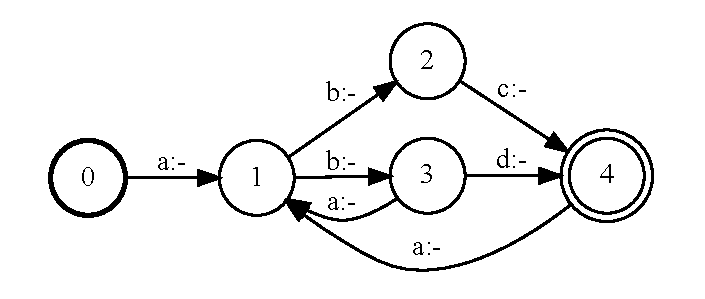
\includegraphics[width=0.5\linewidth]{\imagesPath/ex3-1a.pdf}
					\caption{Το αρχικό αυτόματο (δεν αναγράφονται βάρη/έξοδοι)}
				\end{center}
			\end{figure}
			
			\begin{figure}[H]
				\begin{center}
					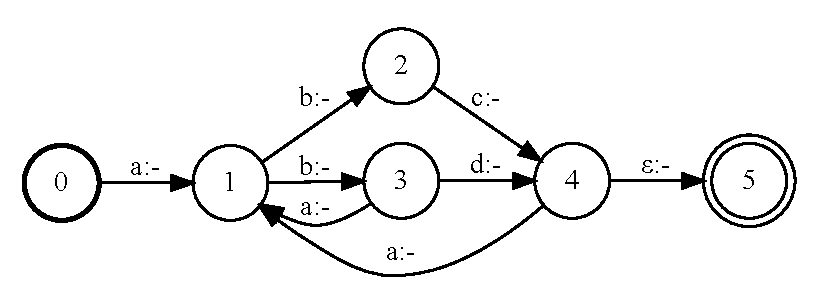
\includegraphics[width=0.5\linewidth]{\imagesPath/ex3-1b.pdf}
					\caption{Προσθέσαμε την κατάσταση 5 επειδή είχαμε απερχόμενες ακμές από την 4}
				\end{center}
			\end{figure}

			\begin{figure}[H]
				\begin{center}
					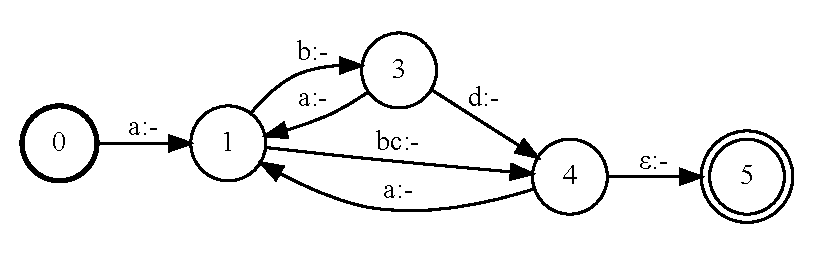
\includegraphics[width=0.5\linewidth]{\imagesPath/ex3-1c.pdf}
					\caption{Ύστερα από διαγραφή της κατάστασης 2}
				\end{center}
			\end{figure}

			\begin{figure}[H]
				\begin{center}
					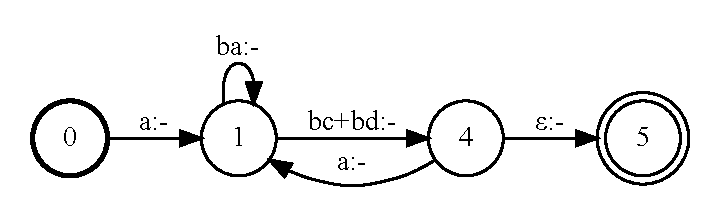
\includegraphics[width=0.5\linewidth]{\imagesPath/ex3-1d.pdf}
					\caption{Ύστερα από διαγραφή της κατάστασης 3}
				\end{center}
			\end{figure}

			\begin{figure}[H]
				\begin{center}
					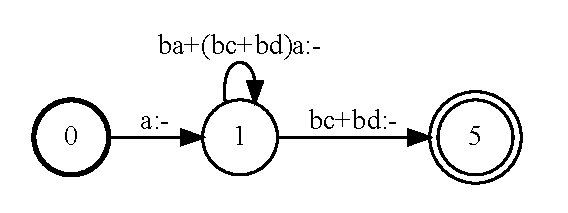
\includegraphics[width=0.5\linewidth]{\imagesPath/ex3-1e.pdf}
					\caption{Ύστερα από διαγραφή της κατάστασης 4}
				\end{center}
			\end{figure}

			\begin{figure}[H]
				\begin{center}
					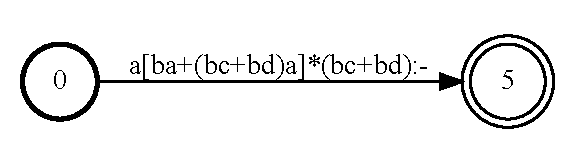
\includegraphics[width=0.5\linewidth]{\imagesPath/ex3-1f}
					\caption{Τελικό αυτόματο, ύστερα από διαγραφή της κατάστασης 1}
				\end{center}
			\end{figure}
			
			Τελικά η κανονική έκφραση που αντιστοιχεί στη μηχανή είναι η:
			
			\[
				a(ba + bca + bda)^*(bc+bd)
			\]
			
			
		\subsubsection*{2.} 
			Τα μονοπάτια που μπορούμε να ακολουθήσουμε (χωρίς να κάνουμε κύκλους, αφού θέλουμε να φτάσουμε σε τελική κατάσταση με το μικρότερο κόστος και όλα τα βάρη είναι θετικά) είναι:
			
			\begin{itemize}
				\item 0 $\rightarrow$ 1 $\rightarrow$ 2 $\rightarrow$ 4 (συμβολοσειρά "abc")
				\item 0 $\rightarrow$ 1 $\rightarrow$ 3 $\rightarrow$ 4 (συμβολοσειρά "abd")
			\end{itemize}
			
			και επειδή χρησιμοποιούμε τον τροπικό ημιδακτύλιο ($\bigoplus$ $\rightarrow$ $\text{min}$, $\bigotimes$ $\rightarrow$ $+$), τα κόστη των συμβολοσειρών θα είναι αντίστοιχα:
			
			\begin{itemize}
				\item 2 $\bigotimes$ 1.5 $\bigotimes$ 2.5 = 2 + 1.5 + 2.5 = 6
				\item 2 $\bigotimes$ 1 $\bigotimes$ 3 = 2 + 1 + 3 = 6
			\end{itemize}
			
			Επομένως οι δύο πιο πιθανές συμβολοσειρές είναι οι "abc" και "abd".
			
		\subsubsection*{3.} 
			Για να φτάσουμε στην γραμματοσειρά "abcababd" ακολουθάμε όλα τα πιθανά μονοπάτια και από αυτά παίρνουμε αυτό με το ελάχιστο αθροιστικό κόστος.
			
			\begin{itemize}
				\item 0 $\xrightarrow{a}$ 1 $\xrightarrow{b}$ 2 $\xrightarrow{c}$ 4 $\xrightarrow{a}$ 1 $\xrightarrow{b}$ 2 (σταματάμε, δεν υπάρχει έγκυρη μετάβαση με είσοδο a).
				\item 0 $\xrightarrow{a}$ 1 $\xrightarrow{b}$ 2 $\xrightarrow{c}$ 4 $\xrightarrow{a}$ 1 $\xrightarrow{b}$ 3 $\xrightarrow{a}$ 1 $\xrightarrow{b}$ 2 (σταματάμε, δεν υπάρχει έγκυρη μετάβαση με είσοδο d)
				\item 0 $\xrightarrow{a}$ 1 $\xrightarrow{b}$ 2 $\xrightarrow{c}$ 4 $\xrightarrow{a}$ 1 $\xrightarrow{b}$ 3 $\xrightarrow{a}$ 1 $\xrightarrow{b}$ 3 $\xrightarrow{d}$ 4 (έγκυρο μονοπάτι)
				\item 0 $\xrightarrow{a}$ 1 $\xrightarrow{b}$ 3 (σταματάμε, δεν υπάρχει έγκυρη μετάβαση με είσοδο c)
			\end{itemize}
			
			Τελικά το μόνο έγκυρο μονοπάτι είναι το τρίτο στη σειρά, με συνολικό κόστος:
			
			\[
				 2 + 1.5 + 2.5 + 1 + 1 + 1 + 1 + 3 = 13,
			\]
			
			που είναι και το κόστος της γραμματοσειράς "abcababd".
		
		\subsubsection*{4.} 
			Η ισοδύναμη ντετερμινιστική μηχανή χωρίς κόστος προκύπτει αν ενώσουμε τις καταστάσεις 2 και 3 σε μία κατάσταση. Μετονομάζουμε τις καταστάσεις έτσι ώστε:
			
			\begin{itemize}
				\item Η 0 παραμένει 0
				\item Η 1 παραμένει 1
				\item Η 2 ενώνεται με την 3 και σχηματίζουν την \textbf{2}
				\item Η 4 μετονομάζεται σε \textbf{3}
			\end{itemize}
			
			Η μηχανή που προκύπτει είναι η εξής:
			
			\begin{figure}[H]
				\begin{center}
					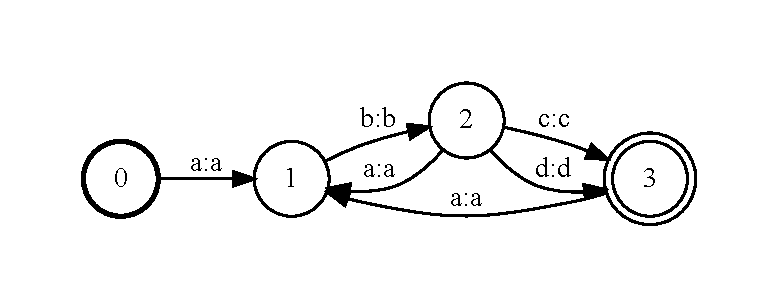
\includegraphics[width=0.75\linewidth]{\imagesPath/ex3-4-raw.pdf}
				\end{center}
			\end{figure}
		
		\subsubsection*{5.} 
			Πρέπει τα κόστη των μονοπατιών να είναι ίδια με την μη-ντετερμινιστική μηχανή. Συγκεκριμένα μας ενδιαφέρουν οι περιπτώσεις των μονοπατιών που περνάνε από τις καταστάσεις 2 και 3 που ενώσαμε. Επομένως έχουμε:
			
			\begin{figure}[H]
				\begin{center}
					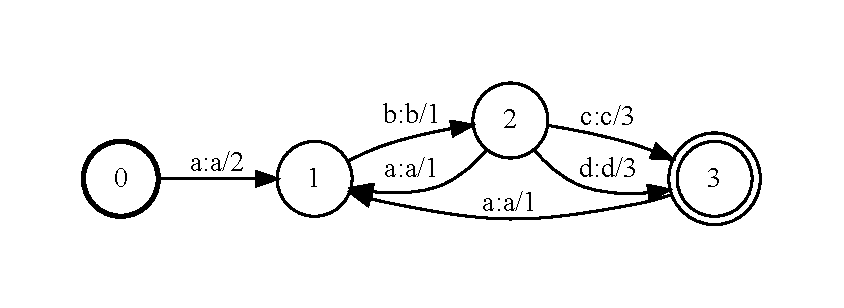
\includegraphics[width=0.75\linewidth]{\imagesPath/ex3-5-raw.pdf}
				\end{center}
			\end{figure}
			

	\subsection*{Άσκηση 4}
	
		\subsubsection*{1.} 
			Ο Levenshtein transducer φαίνεται παρακάτω. Επειδή το πλήθος των μεταβάσεων δυσκολεύει πολύ την οπτικοποίηση, παραθέτουμε και το \verb|.fst| αρχείο που χρησιμοποιήσαμε για πληρότητα: \\
			
			0 0 A A 0 \\
			0 0 A B 1 \\
			0 0 A C 1 \\
			0 0 A D 1 \\
			0 0 A E 1 \\
			0 0 A F 1 \\
			0 0 ε A 1 \\
			0 0 A ε 1 \\
			0 0 B A 1 \\
			0 0 B B 0 \\
			0 0 B C 1 \\
			0 0 B D 1 \\
			0 0 B E 1 \\
			0 0 B F 1 \\
			0 0 B ε 1 \\
			0 0 ε B 1 \\
			0 0 C A 1 \\
			0 0 C B 1 \\
			0 0 C C 0 \\
			0 0 C D 1 \\
			0 0 C E 1 \\
			0 0 C F 1 \\
			0 0 C ε 1 \\
			0 0 ε C 1 \\
			0 0 D A 1 \\
			0 0 D B 1 \\
			0 0 D C 1 \\
			0 0 D D 0 \\
			0 0 D E 1 \\
			0 0 D F 1 \\
			0 0 D ε 1 \\
			0 0 ε D 1 \\
			0 0 E A 1 \\
			0 0 E B 1 \\
			0 0 E C 1 \\
			0 0 E D 1 \\
			0 0 E E 0 \\
			0 0 E F 1 \\
			0 0 E ε 1 \\
			0 0 ε E 1 \\
			0 0 F A 1 \\
			0 0 F B 1 \\
			0 0 F C 1 \\
			0 0 F D 1 \\
			0 0 F E 1 \\
			0 0 F F 0 \\
			0 0 F ε 1 \\
			0 0 ε F 1 \\
			0 \\
			
			
			\begin{figure}[H]
				\begin{center}
					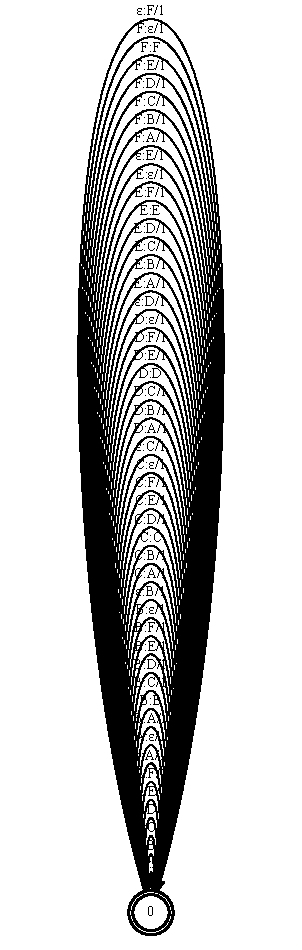
\includegraphics[width=0.4\linewidth]{\imagesPath/ex4-1.pdf}
				\end{center}
			\end{figure}
			
		
		\subsubsection*{2.} 
			Έστω $L$ ο transducer του προηγούμενου ερωτήματος. Για να βρούμε την καλύτερη αντιστοίχιση ανάμεσα στις δύο γραμματοσειρές, φτιάχνουμε δύο transducers $A, B$ που απλά αποδέχονται τις γραμματοσειρές "EDBAEDC" και "CDFABEA" αντίστοιχα (οι ακμές τους επομένως θα έχουν μηδενικό κόστος). 
			
			\begin{figure}[H]
				\begin{center}
					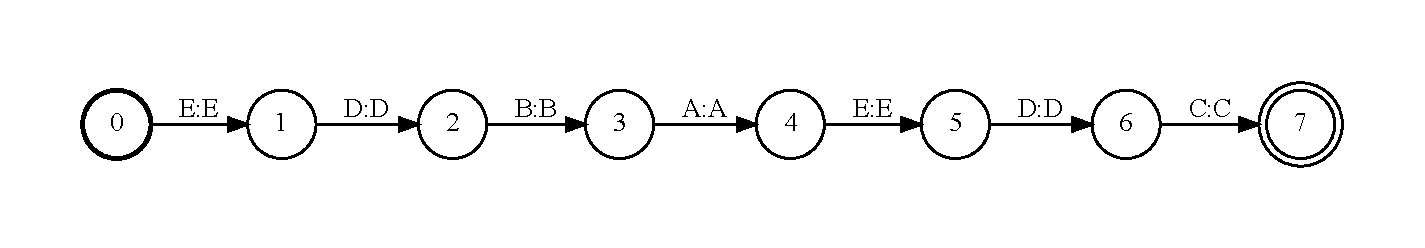
\includegraphics[width=\linewidth]{\imagesPath/ex4-2a-raw.pdf}
					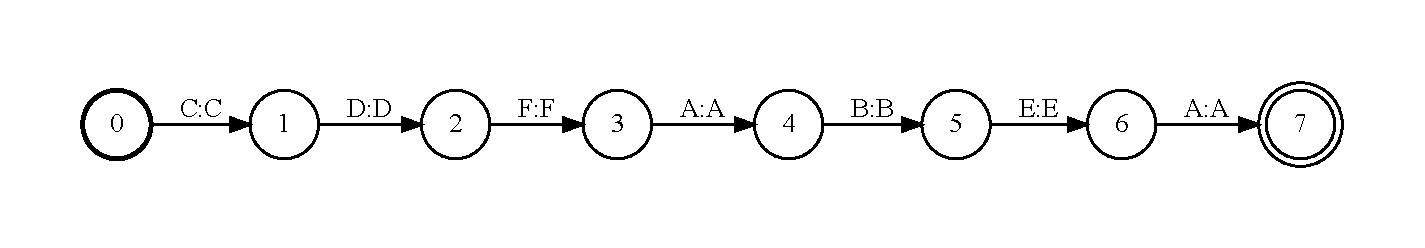
\includegraphics[width=\linewidth]{\imagesPath/ex4-2b-raw.pdf}
				\end{center}
			\end{figure}
			
			Έτσι, το συντομότερο μονοπάτι της σύνθεσης $A \circ L \circ B$ μας δίνει την καλύτερη αντιστοίχιση (για εκτέλεση στο χέρι θα προτιμούσαμε κάποιον αλγόριθμο για min edit distance που χρησιμοποιεί δυναμικό προγραμματισμό, αλλά σκοπός εδώ είναι να φανεί η χρησιμότητα του $L$). Σχεδιάζουμε τις μηχανές $A \circ L$ και $A \circ L \circ B$ (πρώτη και δεύτερη αντίστοιχα) για καλύτερη εποπτεία (οι εικόνες μπορούν να υποστούν μεγάλο ζουμ χωρίς να χαλάσει η ανάλυσή τους):
			
			\begin{figure}[H]
				\begin{center}
					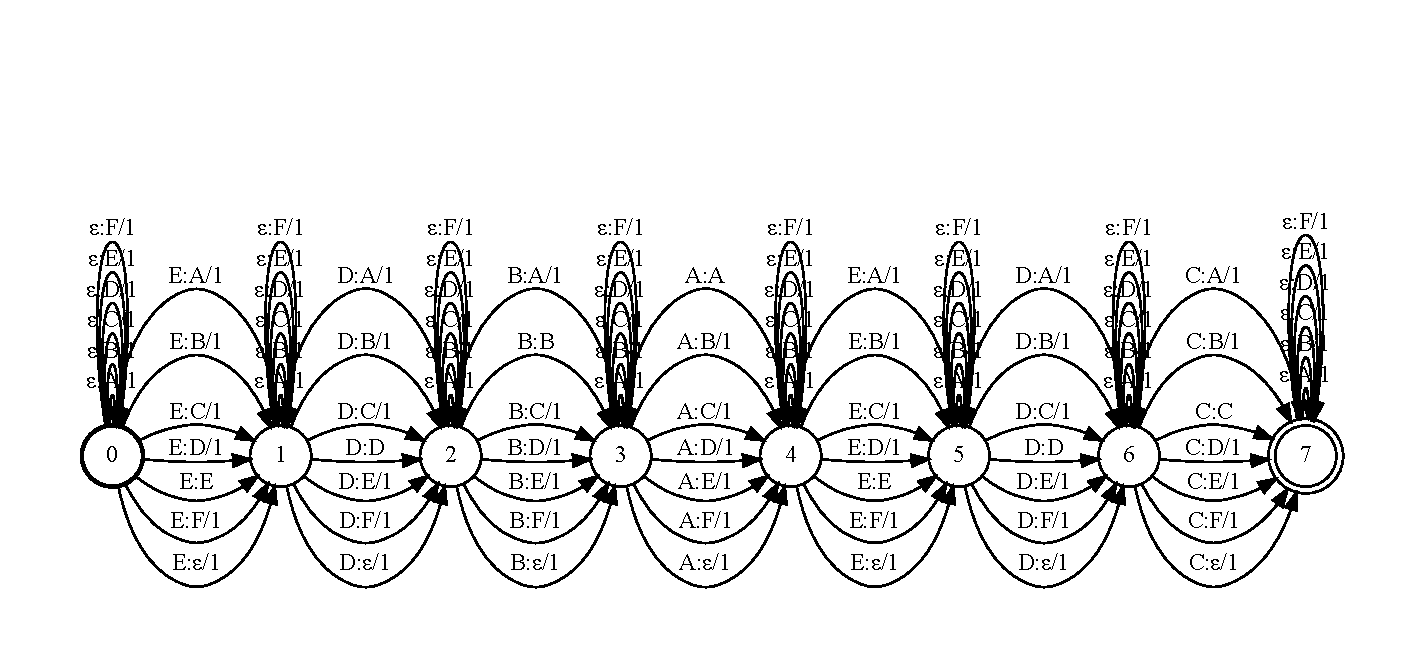
\includegraphics[width=\linewidth]{\imagesPath/ex4-2-comp1-raw.pdf}
				\end{center}
			\end{figure}

			\begin{figure}[H]
				\begin{center}
					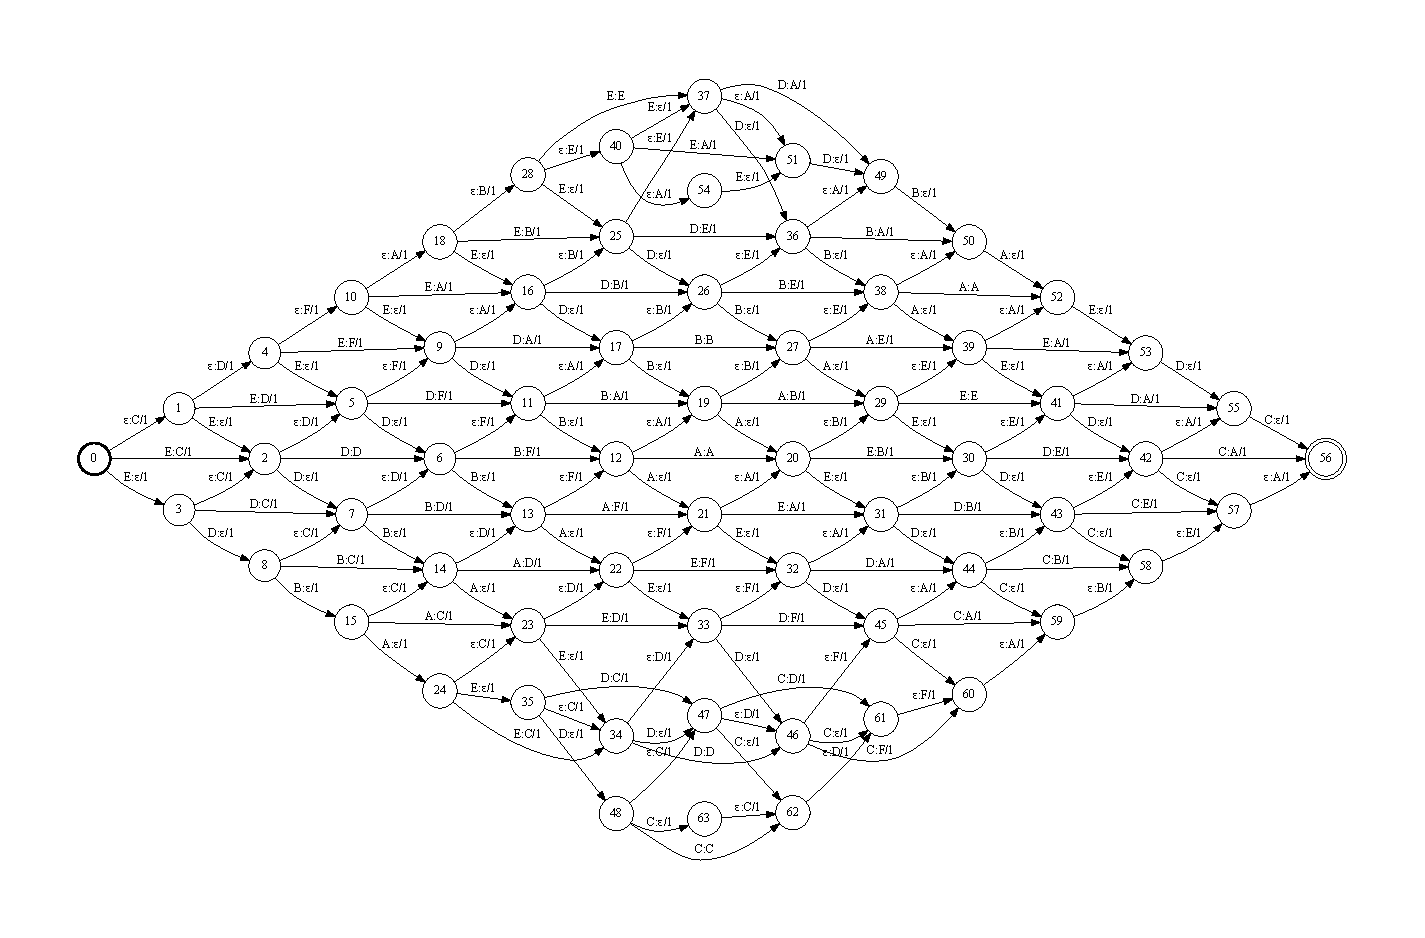
\includegraphics[width=\linewidth]{\imagesPath/ex4-2-comp2-raw.pdf}
				\end{center}
			\end{figure}
		
			Το συντομότερο μονοπάτι στην σύνθεση $A \circ L \circ B$ είναι:
			
			\[
				0 \xrightarrow{E:C/1} 2 \xrightarrow{D:D/0} 6 \xrightarrow{B:F/1} 12 \xrightarrow{A:A/0} 20 \xrightarrow{E:B/1} 30 \xrightarrow{D:E/1} 42 \xrightarrow{C:A/1} 56
			\]
			
			όπου η αρίθμηση έχει ληφθεί από την εικόνα της σύνθεσης $A \circ L \circ B$. Χρειάζονται επομένως 5 edits κατ'ελάχιστον (ο χαρακτήρας που υφίσταται edit κάθε φορά είναι υπογραμμισμένος):
			
			\begin{align*}
				\underline E D B A E D C &\xrightarrow{E \rightarrow C} \\
				C D \underline B A E D C &\xrightarrow{B \rightarrow F} \\
				C D F A \underline E D C &\xrightarrow{E \rightarrow B} \\
				C D F A B \underline D C &\xrightarrow{D \rightarrow E} \\
				C D F A B E \underline C &\xrightarrow{C \rightarrow A} \\
				C D F A B E A
			\end{align*}
		
		\subsubsection*{3.} 
			Το δεύτερο συντομότερο μονοπάτι είναι:
			
			\[
				0 \xrightarrow{E:C/1} 2 \xrightarrow{D:D/0} 6 \xrightarrow{B:F/1} 12 \xrightarrow{A:A/0} 20 \xrightarrow{\epsilon:B/1} 29 \xrightarrow{E:E/0} 41 \xrightarrow{D:\epsilon/1} 42 \xrightarrow{C:A/1} 56
			\]
			
			και πάλι χρειαζόμαστε 5 edits. Η διαδικασία είναι όμοια με παραπάνω.			

	\subsection*{Άσκηση 5}
		
		\subsubsection*{1.} 
			Εξετάζουμε τα τμήματα προτάσεων για να δούμε το πλήθος εμφανίσεων των λέξεων του $L$ καθώς και όλων των ζευγαριών της μορφής $\left\{(w_1, w_2) : w_1, w_2 \in L\right\}$. Θεωρούμε ότι οι διπλότυπες προτάσεις εμφανίζονται η μία αμέσως μετά την άλλη, σύμφωνα με τη \href{https://github.com/slp-ntua/slp-labs/issues/80}{διευκρίνιση} που δόθηκε. 
			
			Αναφερόμαστε στις προτάσεις με έναν αύξοντα αριθμό για ευκολία:
			
			\begin{itemize}
				\item Πρόταση 1: lovely mother grand grandmother lovely grandmother grand mother
				\item Πρόταση 2: lovely mother lovely grandmother lovely
				\item Πρόταση 3: mother grandmother mother
				\item Πρόταση 4: lovely grand lovely
			\end{itemize}
			
			Υπολογίζουμε πόσες εμφανίσεις κάθε λέξης/φράσης οφείλονται στην κάθε πρόταση: \\
			
			\begin{tabular}{|c|c|c|c|c||c|}
				\hline
				\textbf{Λέξη/Φράση} & \textbf{Πρόταση 1} & \textbf{Πρόταση 2} & \textbf{Πρόταση 3} & \textbf{Πρόταση 4} & \textbf{Σύνολο} \\
				\hline
				\hline
				lovely & \textbf{10} & \textbf{21} & 0 & \textbf{2} & \textbf{33} \\
				\hline
				grand & \textbf{10} & 0 & 0 & \textbf{1} & \textbf{11} \\
				\hline
				mother & \textbf{10} & \textbf{7} & \textbf{4} & 0 & \textbf{21} \\
				\hline
				grandmother & \textbf{10} & \textbf{7} & \textbf{2} & 0 & \textbf{19} \\
				\hline
				
				lovely lovely & 0 & \textbf{6} & 0 & 0 & \textbf{6} \\
				\hline
				lovely grand & 0 & 0 & 0 & \textbf{1} & \textbf{1} \\
				\hline
				lovely mother & \textbf{5} & \textbf{7} & 0 & 0 & \textbf{12} \\
				\hline
				lovely grandmother & \textbf{5} & \textbf{7} & 0 & 0 & \textbf{12} \\
				\hline
				
				grand lovely & 0 & 0 & 0 & \textbf{1} & \textbf{1} \\
				\hline
				grand grand & 0 & 0 & 0 & 0 & \textbf{0} \\
				\hline
				grand mother & \textbf{5} & 0 & 0 & 0 & \textbf{5} \\
				\hline
				grand grandmother & \textbf{5} & 0 & 0 & 0 & \textbf{5} \\
				\hline
				
				mother lovely & \textbf{4} & \textbf{7} & 0 & 0 & \textbf{11} \\
				\hline
				mother grand & \textbf{5} & 0 & 0 & 0 & \textbf{5} \\
				\hline
				mother mother & 0 & 0 & \textbf{1} & 0 & \textbf{1} \\
				\hline
				mother grandmother & 0 & 0 & \textbf{2} & 0 & \textbf{2} \\
				\hline
				
				grandmother lovely & \textbf{5} & \textbf{7} & 0 & 0 & \textbf{12} \\
				\hline
				grandmother grand & \textbf{5} & 0 & 0 & 0 & \textbf{5} \\
				\hline
				grandmother mother & 0 & 0 & \textbf{2} & 0 & \textbf{2} \\
				\hline
				grandmother grandmother & 0 & 0 & 0 & 0 & \textbf{0} \\
				\hline
			\end{tabular}
			 
			Επομένως έχουμε:
			
			\begin{align*}
				\mathbb{P}(\text{lovely}) &= \dfrac{\mathbb{N}(\text{lovely})}{\mathbb{N}(\text{lovely}) + \mathbb{N}(\text{grand}) + \mathbb{N}(\text{mother}) + \mathbb{N}(\text{grandmother})} \\ 
				&= \dfrac{33}{33+11+21+19} = \dfrac{33}{84} \approx 0.393.
			\end{align*}
			
			και ομοίως:
			
			\begin{align*}
				\mathbb{P}(\text{grand}) &= \dfrac{11}{84} \approx 0.131\\
				\mathbb{P}(\text{mother}) &= \dfrac{21}{84} = 0.250\\
				\mathbb{P}(\text{grandmother}) &= \dfrac{19}{84} \approx 0.226 \\
			\end{align*}
			
			Επίσης:
			
			\begin{align*}
				\mathbb{P}(\text{lovely | lovely}) &= \dfrac{\mathbb{N}(\text{lovely lovely})}{\mathbb{N}(\text{lovely})} = \dfrac{6}{33} \approx 0.182 \\
				\mathbb{P}(\text{lovely | grand}) &= \dfrac{\mathbb{N}(\text{lovely grand})}{\mathbb{N}(\text{grand})} = \dfrac{1}{11} \approx 0.091 \\
				\mathbb{P}(\text{lovely | mother}) &= \dfrac{\mathbb{N}(\text{lovely mother})}{\mathbb{N}(\text{mother})} = \dfrac{12}{21} \approx 0.571 \\
				\mathbb{P}(\text{lovely | grandmother}) &= \dfrac{\mathbb{N}(\text{lovely grandmother})}{\mathbb{N}(\text{grandmother})} = \dfrac{12}{19} \approx 0.632 \\
			\end{align*}
			
			και ομοίως:
			
			\begin{align*}
				\mathbb{P}(\text{grand | lovely}) &= \dfrac{1}{33} \approx 0.030 \\
				\mathbb{P}(\text{grand | grand}) &= 0 ~~~~\text{(θα χρησιμοποιήσουμε back-off στη συνέχεια)}\\
				\mathbb{P}(\text{grand | mother}) &= \dfrac{5}{21} \approx 0.238 \\
				\mathbb{P}(\text{grand | grandmother}) &= \dfrac{5}{19} \approx 0.263\\
			\end{align*}
			
			\begin{align*}
				\mathbb{P}(\text{mother | lovely}) &= \dfrac{11}{33} \approx 0.333 \\
				\mathbb{P}(\text{mother | grand}) &= \dfrac{5}{11} \approx 0.455 \\
				\mathbb{P}(\text{mother | mother}) &= \dfrac{1}{21} \approx 0.048 \\
				\mathbb{P}(\text{mother | grandmother}) &= \dfrac{2}{19} \approx 0.105 ~~~~~~~~~~~~~~~~~~~~~~~~~~~~~~~~~~~~~~~~~~~~~~~~~~~~~~~~ \\
			\end{align*}
			
			\begin{align*}
				\mathbb{P}(\text{grandmother | lovely}) &= \dfrac{12}{33} \approx 0.364 \\
				\mathbb{P}(\text{grandmother | grand}) &= \dfrac{5}{11} \approx 0.455 \\
				\mathbb{P}(\text{grandmother | mother}) &= \dfrac{2}{21} \approx 0.095 \\
				\mathbb{P}(\text{grandmother | grandmother}) &= 0 ~~~~(\text{θα χρησιμοποιήσουμε back-off στη συνέχεια}) \\
			\end{align*}
			
			Επειδή οι πιθανότητες $~\mathbb{P}(\text{grand | grand})~$ και $~\mathbb{P}(\text{grandmother | grandmother})~$ βγαίνουν μηδενικές, θα χρησιμοποιήσουμε back-off. \\
			
			Για το $~\mathbb{P}(\text{grand | grand})~$:
			
			\begin{align*}
				a &= 1 - \mathbb{P}(\text{grand | lovely}) - \mathbb{P}(\text{grand | mother}) - \mathbb{P}(\text{grand | grandmother}) \\
				&= 1 - 0.030 - 0.238 - 0.263 \\
				&= 0.469
			\end{align*}
			
			Επομένως:
			\[
				\mathbb{P}(\text{grand | grand}) = a \cdot \mathbb{P}(\text{grand}) = 0.469 \cdot 0.131 = 0.061 
			\] \\
			
			Για το $~\mathbb{P}(\text{grandmother | grandmother})~$:
			
			\begin{align*}
				a' &= 1 - \mathbb{P}(\text{grandmother | lovely}) - \mathbb{P}(\text{grandmother | grand}) - \mathbb{P}(\text{grandmother | mother}) \\
				&= 1 - 0.364 - 0.455 - 0.095 \\ 
				&= 0.086
			\end{align*} \\
			
			Επομένως: 
			\[
				\mathbb{P}(\text{grandmother | grandmother}) = a' \cdot \mathbb{P}(\text{grandmother}) = 0.086 \cdot 0.226 = 0.019 
			\]
			
			Σχεδιάζουμε την μηχανή πεπερασμένης κατάστασης με κόστος $-\text{log}P$ (δεκαδικός λογάριθμος). Οι παύλες δεν έχουν κάποιο συγκεκριμένο νόημα, απλά δείχνουν πως δεν μας ενδιαφέρει η έξοδος στην συγκεκριμένη περίπτωση. Η εικόνα της μηχανής μπορεί να υποστεί αρκετό ζουμ χωρίς να αλλοιωθεί η ανάλυση. Οι καταστάσεις είναι αριθμημένες έτσι ώστε:
			
			\begin{itemize}
				\item Η κατάσταση 0 να είναι η αρχική κατάσταση
				\item Η κατάσταση 1 να δείχνει ότι η πιο πρόσφατη λέξη που διαβάστηκε είναι "lovely"
				\item Η κατάσταση 2 να δείχνει ότι η πιο πρόσφατη λέξη που διαβάστηκε είναι "grand"
				\item Η κατάσταση 3 να δείχνει ότι η πιο πρόσφατη λέξη που διαβάστηκε είναι "mother"
				\item Η κατάσταση 4 να δείχνει ότι η πιο πρόσφατη λέξη που διαβάστηκε είναι "grandmother"
			\end{itemize}
			
			\begin{figure}[H]
				\begin{center}
					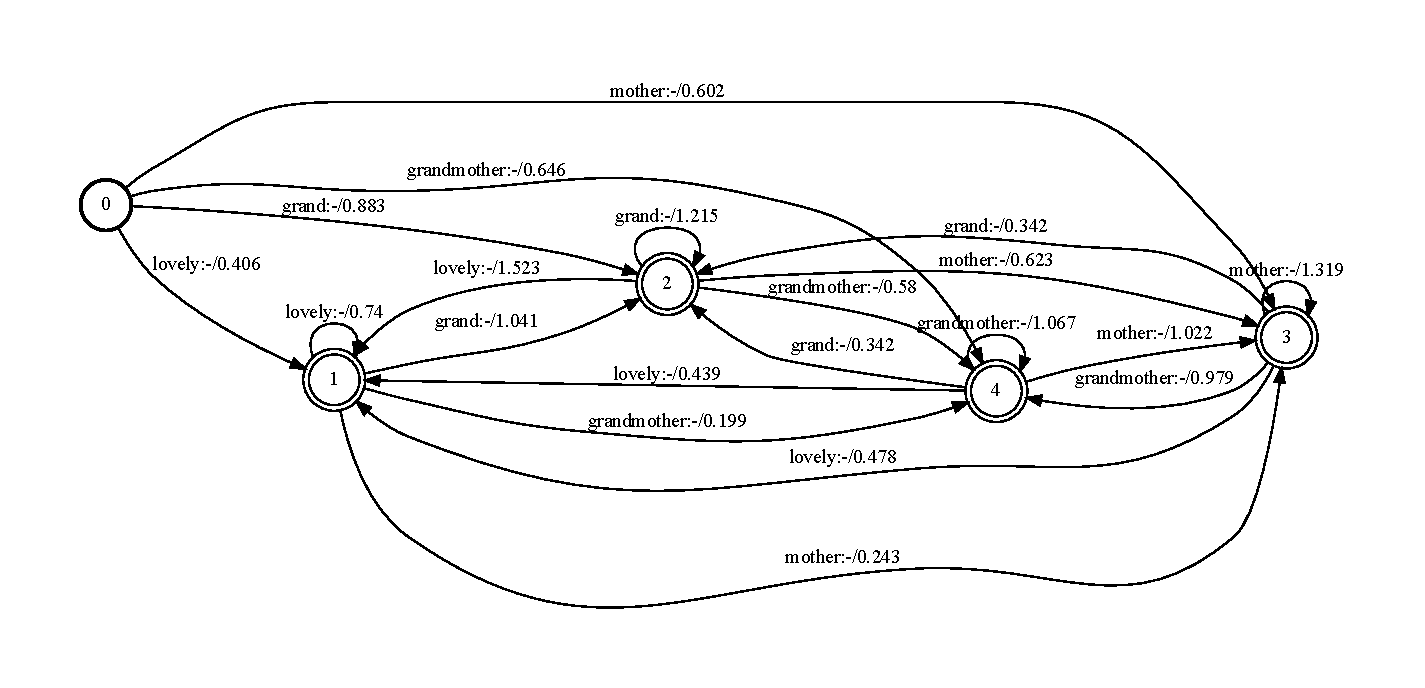
\includegraphics[width=\linewidth]{\imagesPath/ex5-1-raw.pdf}
				\end{center}
			\end{figure}
			
		
		\subsubsection*{2.} 
			Δεδομένης της εισόδου "lovelygrandmothergrandmother", υπάρχουν πολλοί τρόποι να χωριστεί αυτή σε έγκυρες λέξεις του λεξικού. Όλοι αυτοί οι τρόποι απεικονίζονται με το ακόλουθο δέντρο μονοπατιών, όπου τα βάρη έχουν κόστος $-\text{log}P$ όπως και πριν:
		
			\begin{figure}[H]
				\begin{center}
					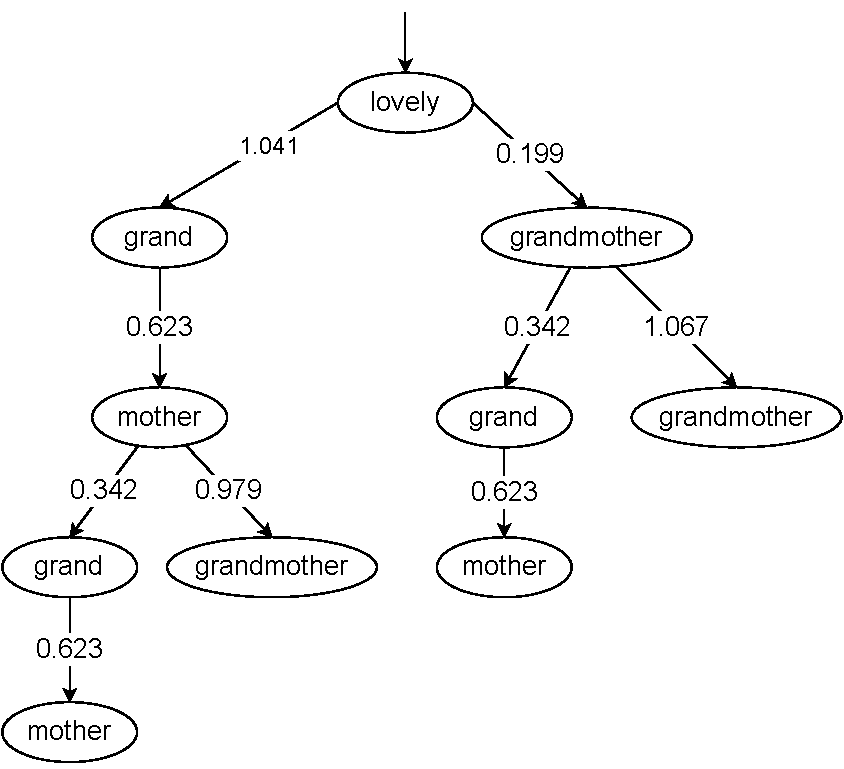
\includegraphics[width=0.6\linewidth]{\imagesPath/ex5-2.pdf}
				\end{center}
			\end{figure}
			
			Η πιθανότερη σειρά από λέξεις είναι αυτή που θα έχει μικρότερο αθροιστικό κόστος στο παραπάνω δέντρο. Παρακάτω φαίνονται οι πιθανές σειρές λέξεων ταξινομημένες από την πιο πιθανή στην λιγότερη πιθανή:
			
			\begin{itemize}
				\item lovely grandmother grand mother $\rightarrow$ 0.199 + 0.342 + 0.623 = 1.164
				\item lovely grandmother grandmother $\rightarrow$ 0.199 + 1.067 = 1.266
				\item lovely grand mother grand mother $\rightarrow$ 1.041 + 0.623 + 0.342 + 0.623 = 2.629
				\item lovely grand mother grandmother $\rightarrow$ 1.041 + 0.623 + 0.979 = 2.643
			\end{itemize}
			
			Τελικά η πιο πιθανή σειρά από λέξεις είναι η \textbf{lovely grandmother grand mother}.
			
	\subsection*{Άσκηση 6}
		Το cepstrum ορίζεται ως:
		
		\begin{align*}
			\hat v(n) &= \mathcal{Z}^{-1} \left\{ \text{log} V(z) \right\} 
		\end{align*}
		
		Έχουμε:
		
		\begin{align*}
			\text{log} V(z) &= \text{log} \dfrac{1}{\prod_{k=1}^{q} (1-c_kz^{-1})(1-c_k^*z^{-1})} \\
			&= -\text{log} \prod_{k=1}^{q} (1-c_kz^{-1})(1-c_k^*z^{-1}) \\
			&= -\sum_{k=1}^{q} \text{log} (1-c_kz^{-1})(1-c_k^*z^{-1}) \\
			&= -\sum_{k=1}^{q} \left[ \text{log} (1-c_kz^{-1}) + \text{log} (1-c_k^*z^{-1}) \right] \\
			&= -\sum_{k=1}^{q} \left[ -\sum_{n=1}^{\infty} \dfrac{\left(c_kz^{-1}\right)^n}{n} -\sum_{n=1}^{\infty} \dfrac{\left(c_k^*z^{-1}\right)^n}{n} \right] \left(\text{επειδή } \text{log} (1-x) = -\sum_{n=1}^{\infty} \dfrac{x^n}{n}\right) \\
			&= \sum_{k=1}^{q} \sum_{n=1}^{\infty} \dfrac{c_k^n+\left(c_k^*\right)^n}{n} \cdot z^{-n} \\
			&= \sum_{n=1}^{\infty} \sum_{k=1}^{q} \dfrac{c_k^n+\left(c_k^*\right)^n}{n} \cdot z^{-n} \\
			&= \sum_{n=1}^{\infty} \sum_{k=1}^{q} \dfrac{r_k^ne^{j\theta_kn}+r_k^ne^{-j\theta_kn}}{n}z^{-n} \\
		\end{align*}
		
		Έχουμε φέρει το αποτέλεσμα στη μορφή του ορισμού του μετασχηματισμού Z:
		
		\begin{align*}
			\sum_{n=-\infty}^{\infty} \hat v(n) z^{-n}
		\end{align*}
		
		όπου:
		
		\begin{align*}
			\hat v(n) &= \sum_{k=1}^{q} \dfrac{r_k^ne^{j\theta_kn}+r_k^ne^{-j\theta_kn}}{n} \\
			&= \sum_{k=1}^{q} \dfrac{r_k^n}{n}\left(e^{j\theta_kn}+e^{-j\theta_kn}\right) \\
			&= 2 \sum_{k=1}^{q} \dfrac{r_k^n}{n} \cos(\theta_k n), \text{ για } n > 0, \\
		\end{align*}
		
		που είναι και το ζητούμενο.
\end{document}